\documentclass{beamer}
\usetheme{Boadilla}
\setbeamertemplate{caption}[numbered]

\usepackage{natbib}
\usepackage{xcolor}
\usepackage{booktabs}
\usepackage{adjustbox}
\usepackage{appendixnumberbeamer}
\bibliographystyle{apalike}

\newcommand{\red}[1]{\textcolor{red}{#1}}
\newcommand{\blue}[1]{\textcolor{blue}{#1}}

\defcitealias{myers1984corporate}{MM84}
\defcitealias{gertner1994internal}{GSS94}
\defcitealias{holmstrom1998private}{HT98}
\defcitealias{brunnermeier2009market}{BP09}
\defcitealias{he2013intermediary}{HK13}
\defcitealias{diamond1983bank}{DD83}
\defcitealias{diamond1984financial}{D84}
\defcitealias{gorton1990financial}{GP90}
\defcitealias{hanson2015banks}{HSSV15}
\defcitealias{kashyap2002banks}{KRS02}
\defcitealias{holmstrom1997financial}{HT97}
\defcitealias{bolton2011outside}{BSS11}

\title[Youth and redistribution]{Why do young Americans support redistribution?}
\subtitle{Survey evidence on a widening U.S. age gap}
% Documenting a widening U.S. age gap and its drivers

\author[Carlson and Rancière]{Niclas Carlson and Romain Rancière}
% \institute{Columbia Business School}
\date{\today}

\begin{document}


\begin{frame}
\titlepage
\end{frame}



\begin{frame}{Formative-years growth and redistribution in the US}

\begin{table}
    \centering
    \setbeamerfont{caption}{size=\footnotesize}
    \caption{Prolific 2025: support for redistribution on home-state formative-years income growth}
    \vspace{-1.1em}
    {\tiny\setlength{\tabcolsep}{4pt}\renewcommand{\arraystretch}{0.82}
          \begin{adjustbox}{max width=\linewidth}
   \begin{tabular}{lcccccc}
      \tabularnewline \midrule \midrule
      Dependent Variables: & \multicolumn{4}{c}{Reduce income differences} & \shortstack{More progressive\\ taxes} & \shortstack{Support redistributive\\ proposal}\\
      Spec.: & 0--20 & 18--25 & 0--20, $+$age & 0--20, $+$coh. & \multicolumn{2}{c}{0--20} \\ 
      Model:                        & (1)            & (2)     & (3)                   & (4)     & (5)            & (6)\\  
      \midrule
      \emph{Variables}\\
      Formative growth, ages 0--20  & -0.281$^{***}$ &         & 0.082                 & 0.028   & -0.143$^{***}$ & -0.152$^{***}$\\   
                                    & (0.045)        &         & (0.059)               & (0.071) & (0.043)        & (0.042)\\   
      Formative growth, ages 18--25 &                & -0.002  &                       &         &                &   \\   
                                    &                & (0.026) &                       &         &                &   \\   
      Age                           &                &         & -0.019$^{**}$         &         &                &   \\   
                                    &                &         & (0.009)               &         &                &   \\   
      Age$^2$                       &                &         & $4.21\times 10^{-5}$  &         &                &   \\   
                                    &                &         & (0.0001)              &         &                &   \\   
      \midrule
      \emph{Fixed-effects}\\
      Home state                    & Yes            & Yes     & Yes                   & Yes     & Yes            & Yes\\  
      Birth year (cohort)           &                &         &                       & Yes     &                & \\  
      \midrule
      \emph{Fit statistics}\\
      Observations                  & 2,231          & 1,802   & 2,231                 & 2,231   & 2,231          & 2,231\\  
      R$^2$                         & 0.03980        & 0.02467 & 0.07179               & 0.10113 & 0.02824        & 0.02554\\  
      \midrule \midrule
      \multicolumn{7}{l}{\emph{Clustered (Home state) standard-errors in parentheses}}\\
      \multicolumn{7}{l}{\emph{Signif. Codes: ***: 0.01, **: 0.05, *: 0.1}}\\
   \end{tabular}
      \end{adjustbox}
\vspace{3pt}\par\centering{\setlength{\tabcolsep}{4pt}
\begin{tabular}{lcccccc}
\multicolumn{1}{l}{\itshape Economic size (significant columns only):}
 & (1) & (2) & (3) & (4) & (5) & (6)\\
\midrule
Per $+1$\,SD of regressor ($\Delta$ outcome, SD) & $-0.150$ & -- & -- & -- & $-0.077$ & $-0.081$\\
\quad as \% of the young--old gap & 57\% & -- & -- & -- & 55\% & 61\%\\
\end{tabular}}
}
\end{table}

\end{frame}



\begin{frame}{Formative-years growth and redistribution: movers only}

\begin{table}
    \centering
    \setbeamerfont{caption}{size=\footnotesize}
    \caption{Prolific 2025, movers only (home state $\neq$ current state): support for redistribution on home-state formative growth, with and without current-state FE}
    \vspace{-1.1em}
    {\tiny\setlength{\tabcolsep}{5pt}\renewcommand{\arraystretch}{0.82}
       \begin{tabular}{lcccc}
      \tabularnewline \midrule \midrule
      Dependent Variable: & \multicolumn{4}{c}{Reduce income differences}\\
      Current-state FE:            & No             & Yes            & No       & Yes \\   
      Age controls: & \multicolumn{2}{c}{No} & \multicolumn{2}{c}{Yes} \\ 
      Model:                       & (1)            & (2)            & (3)      & (4)\\  
      \midrule
      \emph{Variables}\\
      Formative growth, ages 0--20 & -0.338$^{***}$ & -0.312$^{***}$ & 0.032    & 0.071\\   
                                   & (0.071)        & (0.079)        & (0.108)  & (0.117)\\   
      Age                          &                &                & -0.030   & -0.024\\   
                                   &                &                & (0.021)  & (0.022)\\   
      Age$^2$                      &                &                & 0.0002   & $9.08\times 10^{-5}$\\    
                                   &                &                & (0.0002) & (0.0003)\\   
      \midrule
      \emph{Fixed-effects}\\
      Home state                   & Yes            & Yes            & Yes      & Yes\\  
      Current state                &                & Yes            &          & Yes\\  
      \midrule
      \emph{Fit statistics}\\
      Observations                 & 673            & 672            & 673      & 672\\  
      R$^2$                        & 0.07756        & 0.17744        & 0.10692  & 0.20350\\  
      \midrule \midrule
      \multicolumn{5}{l}{\emph{Clustered (Home state) standard-errors in parentheses}}\\
      \multicolumn{5}{l}{\emph{Signif. Codes: ***: 0.01, **: 0.05, *: 0.1}}\\
   \end{tabular}
\vspace{3pt}\par\centering{\setlength{\tabcolsep}{4pt}
\begin{tabular}{lcccc}
\multicolumn{1}{l}{\itshape Economic size (significant columns only):}
 & (1) & (2) & (3) & (4)\\
\midrule
Per $+1$\,SD of regressor ($\Delta$ outcome, SD) & $-0.198$ & $-0.183$ & -- & --\\
\quad as \% of the young--old gap & 70\% & 64\% & -- & --\\
\end{tabular}}
}
\end{table}

\end{frame}



\begin{frame}{Absolute mobility and redistribution in the US}

\begin{table}
    \centering
    \setbeamerfont{caption}{size=\footnotesize}
    \caption{Prolific 2025: support for redistribution on home-state absolute mobility}
    \vspace{-1.1em}
    {\tiny\setlength{\tabcolsep}{4pt}\renewcommand{\arraystretch}{0.82}
          \begin{adjustbox}{max width=\linewidth}
   \begin{tabular}{lccccc}
      \tabularnewline \midrule \midrule
      Dependent Variables: & \multicolumn{3}{c}{Reduce income differences} & \shortstack{More progressive\\ taxes} & \shortstack{Support redistributive\\ proposal}\\
      Spec.: & home FE & $+$age & $+$coh. & \multicolumn{2}{c}{home FE} \\ 
      Model:                 & (1)            & (2)      & (3)          & (4)     & (5)\\  
      \midrule
      \emph{Variables}\\
      Absolute mobility (SD) & -0.113$^{***}$ & -0.077   & -0.303$^{*}$ & -0.031  & -0.060$^{**}$\\   
                             & (0.034)        & (0.091)  & (0.164)      & (0.044) & (0.028)\\   
      Age                    &                & -0.036   &              &         &   \\   
                             &                & (0.028)  &              &         &   \\   
      Age$^2$                &                & 0.0003   &              &         &   \\   
                             &                & (0.0002) &              &         &   \\   
      \midrule
      \emph{Fixed-effects}\\
      Home state             & Yes            & Yes      & Yes          & Yes     & Yes\\  
      Birth year (cohort)    &                &          & Yes          &         & \\  
      \midrule
      \emph{Fit statistics}\\
      Observations           & 998            & 998      & 998          & 998     & 998\\  
      R$^2$                  & 0.04822        & 0.04990  & 0.09092      & 0.04996 & 0.04385\\  
      \midrule \midrule
      \multicolumn{6}{l}{\emph{Clustered (Home state) standard-errors in parentheses}}\\
      \multicolumn{6}{l}{\emph{Signif. Codes: ***: 0.01, **: 0.05, *: 0.1}}\\
   \end{tabular}
      \end{adjustbox}
\vspace{3pt}\par\centering{\setlength{\tabcolsep}{4pt}
\begin{tabular}{lccccc}
\multicolumn{1}{l}{\itshape Economic size (significant columns only):}
 & (1) & (2) & (3) & (4) & (5)\\
\midrule
Per $+1$\,SD of regressor ($\Delta$ outcome, SD) & $-0.113$ & -- & -- & -- & $-0.060$\\
\quad as \% of the young--old gap & 43\% & -- & -- & -- & 45\%\\
\end{tabular}}
}
\end{table}

\end{frame}



\begin{frame}{Formative-years growth relative to the nation}

\begin{table}
    \centering
    \setbeamerfont{caption}{size=\footnotesize}
    \caption{Prolific 2025: support for redistribution on state$-$national formative growth}
    \vspace{-1.1em}
    {\tiny\setlength{\tabcolsep}{5pt}\renewcommand{\arraystretch}{0.82}
       \begin{tabular}{lcccc}
      \tabularnewline \midrule \midrule
      Dependent Variable: & \multicolumn{4}{c}{Support for redistribution}\\
      Spec.:                               & 0--20   & 18--25  & 0--20, $+$age           & 0--20, $+$coh. \\   
      Model:                               & (1)     & (2)     & (3)                     & (4)\\  
      \midrule
      \emph{Variables}\\
      State$-$national growth, ages 0--20  & 0.021   &         & 0.036                   & 0.028\\   
                                           & (0.174) &         & (0.073)                 & (0.071)\\   
      State$-$national growth, ages 18--25 &         & -0.036  &                         &   \\   
                                           &         & (0.051) &                         &   \\   
      Age                                  &         &         & -0.022$^{**}$           &   \\   
                                           &         &         & (0.009)                 &   \\   
      Age$^2$                              &         &         & $9.05\times 10^{-5}$    &   \\   
                                           &         &         & ($9.97\times 10^{-5}$)  &   \\   
      \midrule
      \emph{Fixed-effects}\\
      State                                & Yes     & Yes     & Yes                     & Yes\\  
      Birth year (cohort)                  &         &         &                         & Yes\\  
      \midrule
      \emph{Fit statistics}\\
      Observations                         & 2,231   & 1,802   & 2,231                   & 2,231\\  
      R$^2$                                & 0.01985 & 0.02504 & 0.07118                 & 0.10113\\  
      \midrule \midrule
      \multicolumn{5}{l}{\emph{Clustered (State) standard-errors in parentheses}}\\
      \multicolumn{5}{l}{\emph{Signif. Codes: ***: 0.01, **: 0.05, *: 0.1}}\\
   \end{tabular}
\vspace{2pt}\par\centering{\itshape Economic size: no coefficient significant at 5\%.}
}
\end{table}

\end{frame}



\begin{frame}{Absolute mobility relative to the nation}

\begin{table}
    \centering
    \setbeamerfont{caption}{size=\footnotesize}
    \caption{Prolific 2025: support for redistribution on state$-$national absolute mobility}
    \vspace{-1.1em}
    {\tiny\setlength{\tabcolsep}{5pt}\renewcommand{\arraystretch}{0.82}
       \begin{tabular}{lccc}
      \tabularnewline \midrule \midrule
      Dependent Variable: & \multicolumn{3}{c}{Support for redistribution}\\
      Spec.:                              & home FE       & $+$age   & $+$coh. \\   
      Model:                              & (1)           & (2)      & (3)\\  
      \midrule
      \emph{Variables}\\
      State$-$national abs. mobility (SD) & -0.124$^{**}$ & -0.025   & -0.126$^{*}$\\   
                                          & (0.047)       & (0.064)  & (0.068)\\   
      Age                                 &               & -0.027   &   \\   
                                          &               & (0.032)  &   \\   
      Age$^2$                             &               & 0.0002   &   \\   
                                          &               & (0.0003) &   \\   
      \midrule
      \emph{Fixed-effects}\\
      State                               & Yes           & Yes      & Yes\\  
      Birth year (cohort)                 &               &          & Yes\\  
      \midrule
      \emph{Fit statistics}\\
      Observations                        & 998           & 998      & 998\\  
      R$^2$                               & 0.04667       & 0.04943  & 0.09092\\  
      \midrule \midrule
      \multicolumn{4}{l}{\emph{Clustered (State) standard-errors in parentheses}}\\
      \multicolumn{4}{l}{\emph{Signif. Codes: ***: 0.01, **: 0.05, *: 0.1}}\\
   \end{tabular}
\vspace{3pt}\par\centering{\setlength{\tabcolsep}{4pt}
\begin{tabular}{lccc}
\multicolumn{1}{l}{\itshape Economic size (significant columns only):}
 & (1) & (2) & (3)\\
\midrule
Per $+1$\,SD of regressor ($\Delta$ outcome, SD) & $-0.124$ & -- & --\\
\quad as \% of the young--old gap & 39\% & -- & --\\
\end{tabular}}
}
\end{table}

\end{frame}



\begin{frame}{Inequality grown up with and redistribution}

\begin{table}
    \centering
    \setbeamerfont{caption}{size=\footnotesize}
    \caption{Prolific 2025: support for redistribution on the top-10\% income share grown up with}
    \vspace{-1.1em}
    {\tiny\setlength{\tabcolsep}{5pt}\renewcommand{\arraystretch}{0.82}
       \begin{tabular}{lcccc}
      \tabularnewline \midrule \midrule
      Dependent Variable: & \multicolumn{4}{c}{concern}\\
                                              & Top10 avg     & Top10 change  & avg $-$ nat & change $-$ nat \\   
      Model:                                  & (1)           & (2)           & (3)         & (4)\\  
      \midrule
      \emph{Variables}\\
      Top-10\% share, formative average (SD)  & 0.265$^{***}$ &               &             &   \\   
                                              & (0.023)       &               &             &   \\   
      Top-10\% share, formative change (SD)   &               & 0.091$^{***}$ &             &   \\   
                                              &               & (0.029)       &             &   \\   
      Formative average $-$ national (SD)     &               &               & -0.041      &   \\   
                                              &               &               & (0.133)     &   \\   
      Formative change $-$ national (SD)      &               &               &             & -0.013\\   
                                              &               &               &             & (0.043)\\   
      \midrule
      \emph{Fixed-effects}\\
      State                                   & Yes           & Yes           & Yes         & Yes\\  
      \midrule
      \emph{Fit statistics}\\
      Observations                            & 2,078         & 2,078         & 2,078       & 2,078\\  
      R$^2$                                   & 0.07168       & 0.02750       & 0.02144     & 0.02121\\  
      \midrule \midrule
      \multicolumn{5}{l}{\emph{Clustered (State) standard-errors in parentheses}}\\
      \multicolumn{5}{l}{\emph{Signif. Codes: ***: 0.01, **: 0.05, *: 0.1}}\\
   \end{tabular}
\vspace{3pt}\par\centering{\setlength{\tabcolsep}{4pt}
\begin{tabular}{lcccc}
\multicolumn{1}{l}{\itshape Economic size (significant columns only):}
 & (1) & (2) & (3) & (4)\\
\midrule
Per $+1$\,SD of regressor ($\Delta$ outcome, SD) & $+0.265$ & $+0.091$ & -- & --\\
\quad as \% of the young--old gap & 97\% & 20\% & -- & --\\
\end{tabular}}
}
\end{table}

\end{frame}



\begin{frame}{Formative-years growth and zero-sum beliefs}

\begin{table}
    \centering
    \setbeamerfont{caption}{size=\footnotesize}
    \caption{Prolific 2025: zero-sum beliefs on home-state formative-years income growth}
    \vspace{-1.1em}
    {\tiny\setlength{\tabcolsep}{4pt}\renewcommand{\arraystretch}{0.82}
          \begin{adjustbox}{max width=\linewidth}
   \begin{tabular}{lcccccc}
      \tabularnewline \midrule \midrule
      Dependent Variables: & \multicolumn{4}{c}{Rich gain at others' expense} & \shortstack{CEO pay at\\ workers' expense} & \shortstack{DEI: opportunity\\ trade-off}\\
      Spec.: & 0--20 & 18--25 & 0--20, $+$age & 0--20, $+$coh. & \multicolumn{2}{c}{0--20} \\ 
      Model:                        & (1)            & (2)     & (3)                    & (4)          & (5)          & (6)\\  
      \midrule
      \emph{Variables}\\
      Formative growth, ages 0--20  & -0.283$^{***}$ &         & 0.107                  & 0.146$^{**}$ & -0.089$^{*}$ & 0.188$^{***}$\\   
                                    & (0.058)        &         & (0.074)                & (0.070)      & (0.046)      & (0.052)\\   
      Formative growth, ages 18--25 &                & 0.051   &                        &              &              &   \\   
                                    &                & (0.031) &                        &              &              &   \\   
      Age                           &                &         & -0.017                 &              &              &   \\   
                                    &                &         & (0.010)                &              &              &   \\   
      Age$^2$                       &                &         & $-1.83\times 10^{-6}$  &              &              &   \\   
                                    &                &         & (0.0001)               &              &              &   \\   
      \midrule
      \emph{Fixed-effects}\\
      Home state                    & Yes            & Yes     & Yes                    & Yes          & Yes          & Yes\\  
      Birth year (cohort)           &                &         &                        & Yes          &              & \\  
      \midrule
      \emph{Fit statistics}\\
      Observations                  & 2,219          & 1,790   & 2,219                  & 2,219        & 2,206        & 2,207\\  
      R$^2$                         & 0.03791        & 0.02769 & 0.07300                & 0.09288      & 0.02284      & 0.03086\\  
      \midrule \midrule
      \multicolumn{7}{l}{\emph{Clustered (Home state) standard-errors in parentheses}}\\
      \multicolumn{7}{l}{\emph{Signif. Codes: ***: 0.01, **: 0.05, *: 0.1}}\\
   \end{tabular}
      \end{adjustbox}
\vspace{3pt}\par\centering{\setlength{\tabcolsep}{4pt}
\begin{tabular}{lcccccc}
\multicolumn{1}{l}{\itshape Economic size (significant columns only):}
 & (1) & (2) & (3) & (4) & (5) & (6)\\
\midrule
Per $+1$\,SD of regressor ($\Delta$ outcome, SD) & $-0.151$ & -- & -- & $+0.078$ & -- & $+0.100$\\
\quad as \% of the young--old gap & 54\% & -- & -- & -28\% & -- & 75\%\\
\end{tabular}}
}
\end{table}

\end{frame}



\begin{frame}{Absolute mobility and zero-sum beliefs}

\begin{table}
    \centering
    \setbeamerfont{caption}{size=\footnotesize}
    \caption{Prolific 2025: zero-sum beliefs on home-state absolute mobility}
    \vspace{-1.1em}
    {\tiny\setlength{\tabcolsep}{4pt}\renewcommand{\arraystretch}{0.82}
          \begin{adjustbox}{max width=\linewidth}
   \begin{tabular}{lccccc}
      \tabularnewline \midrule \midrule
      Dependent Variables: & \multicolumn{3}{c}{Rich gain at others' expense} & \shortstack{CEO pay at\\ workers' expense} & \shortstack{DEI: opportunity\\ trade-off}\\
      Spec.: & home FE & $+$age & $+$coh. & \multicolumn{2}{c}{home FE} \\ 
      Model:                 & (1)            & (2)                   & (3)     & (4)           & (5)\\  
      \midrule
      \emph{Variables}\\
      Absolute mobility (SD) & -0.146$^{***}$ & -0.025                & -0.076  & -0.081$^{**}$ & 0.006\\   
                             & (0.039)        & (0.082)               & (0.211) & (0.031)       & (0.027)\\   
      Age                    &                & -0.018                &         &               &   \\   
                             &                & (0.023)               &         &               &   \\   
      Age$^2$                &                & $6.06\times 10^{-5}$  &         &               &   \\   
                             &                & (0.0002)              &         &               &   \\   
      \midrule
      \emph{Fixed-effects}\\
      Home state             & Yes            & Yes                   & Yes     & Yes           & Yes\\  
      Birth year (cohort)    &                &                       & Yes     &               & \\  
      \midrule
      \emph{Fit statistics}\\
      Observations           & 995            & 995                   & 995     & 988           & 992\\  
      R$^2$                  & 0.06725        & 0.07008               & 0.09496 & 0.05722       & 0.05653\\  
      \midrule \midrule
      \multicolumn{6}{l}{\emph{Clustered (Home state) standard-errors in parentheses}}\\
      \multicolumn{6}{l}{\emph{Signif. Codes: ***: 0.01, **: 0.05, *: 0.1}}\\
   \end{tabular}
      \end{adjustbox}
\vspace{3pt}\par\centering{\setlength{\tabcolsep}{4pt}
\begin{tabular}{lccccc}
\multicolumn{1}{l}{\itshape Economic size (significant columns only):}
 & (1) & (2) & (3) & (4) & (5)\\
\midrule
Per $+1$\,SD of regressor ($\Delta$ outcome, SD) & $-0.146$ & -- & -- & $-0.080$ & --\\
\quad as \% of the young--old gap & 52\% & -- & -- & 108\% & --\\
\end{tabular}}
}
\end{table}

\end{frame}



\begin{frame}{International Evidence}

\begin{figure}
    \centering
    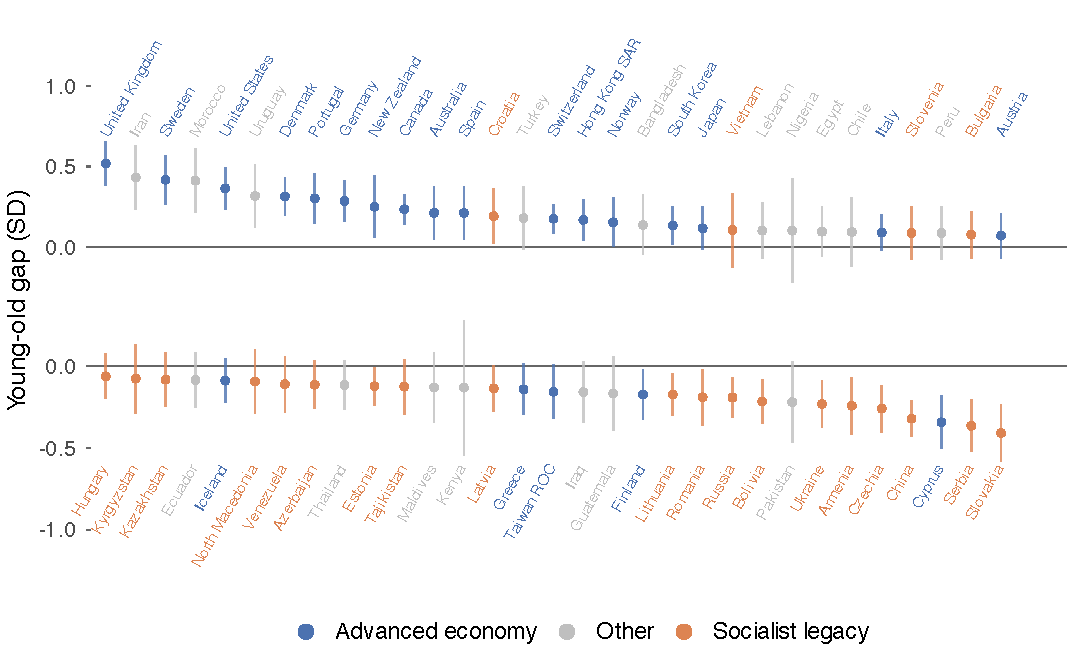
\includegraphics[width=0.85\linewidth]{figures/fig_slide_e037_ends.pdf}
    \caption{\centering Age gap in redistributive preferences in WVS/EVS wave 2017--2022, countries grouped by institutional history}
\end{figure}

\end{frame}



\begin{frame}{Zero-sum beliefs and the age gradient across countries}

\begin{figure}
    \centering
    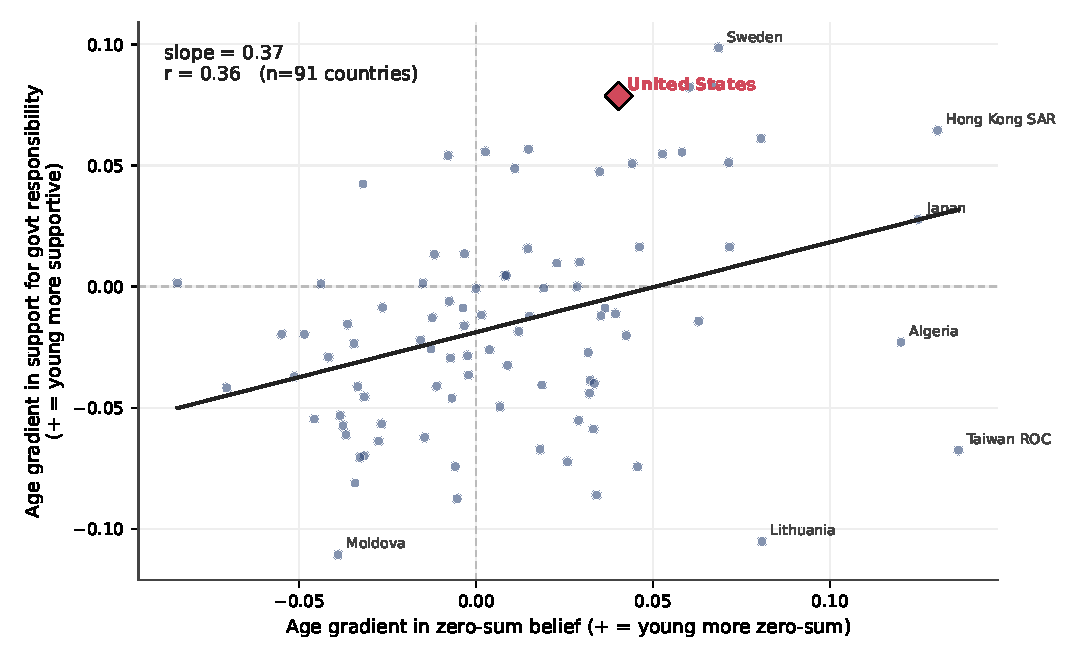
\includegraphics[width=0.7\linewidth]{figures/fig_slide_zerosum_reg_e037.pdf}
    \caption{\centering Age gradient in support for government responsibility (E037) vs.\ age gradient in zero-sum belief (E041), most recent WVS wave per country}
\end{figure}
\vspace{-0.6em}
{\tiny\centering WVS items, 1--10 scales. Government responsibility (E037): 1 = ``People should take more responsibility'' \dots\ 10 = ``The government should take more responsibility''.\\
Zero-sum (E041): 1 = ``People can only get rich at the expense of others'' \dots\ 10 = ``Wealth can grow so there's enough for everyone''.\par}
    
\end{frame}



\begin{frame}{Zero-sum beliefs and redistribution within countries}

\begin{table}
    \centering
    \caption{Individual-level WVS: redistribution on zero-sum belief}
    \vspace{-0.4em}
    {\fontsize{6.5}{7.6}\selectfont\setlength{\tabcolsep}{5pt}\begin{tabular}{lcccc}
\toprule
 & (1) & (2) & (3) & (4) \\
\midrule
\multicolumn{5}{l}{\textit{A. Incomes should be made more equal (\texttt{E035})}} \\
\quad Zero-sum belief (\texttt{E041}) & $0.117^{***}$ & $0.118^{***}$ & $0.107^{***}$ & $0.108^{***}$ \\
 & (0.010) & (0.010) & (0.008) & (0.008) \\
\quad Within $R^2$ & 0.014 & 0.015 & 0.012 & 0.013 \\
\quad Observations & 236,885 & 236,885 & 236,885 & 236,885 \\
\addlinespace
\multicolumn{5}{l}{\textit{B. Government should take more responsibility (\texttt{E037})}} \\
\quad Zero-sum belief (\texttt{E041}) & $0.075^{***}$ & $0.075^{***}$ & $0.068^{***}$ & $0.069^{***}$ \\
 & (0.010) & (0.010) & (0.009) & (0.009) \\
\quad Within $R^2$ & 0.006 & 0.006 & 0.005 & 0.005 \\
\quad Observations & 238,268 & 238,268 & 238,268 & 238,268 \\
\midrule
Country FE & Yes & Yes & & \\
Country $\times$ wave FE & & & Yes & Yes \\
Age control & & Yes & & Yes \\
Countries & 92 & 92 & 92 & 92 \\
\bottomrule
\end{tabular}
}
\end{table}
\vspace{-0.6em}
{\tiny
WVS waves carrying \texttt{E041} (1990--2014), ages 18--79, weighted, SEs clustered by country. Items z-scored over the estimation sample (SD of the outcome per 1 SD of zero-sum); age control is age in decades. * $p<0.05$, ** $p<0.01$, *** $p<0.001$. Items on a 1--10 scale:
\begin{itemize}\setlength{\itemsep}{0pt}
    \item \texttt{E035}: 1 = ``Incomes should be made more equal'' \dots\ 10 = ``We need larger income differences as incentives'' (coded $+$ = pro-equality).
    \item \texttt{E037}: 1 = ``People should take more responsibility'' \dots\ 10 = ``The government should take more responsibility'' (coded $+$ = pro-government).
    \item \texttt{E041}: 1 = ``People can only get rich at the expense of others'' \dots\ 10 = ``Wealth can grow so there's enough for everyone'' (coded $+$ = zero-sum).
\end{itemize}
\par}

\end{frame}



\begin{frame}{The widening age gradient in the US}

\begin{figure}
    \centering
    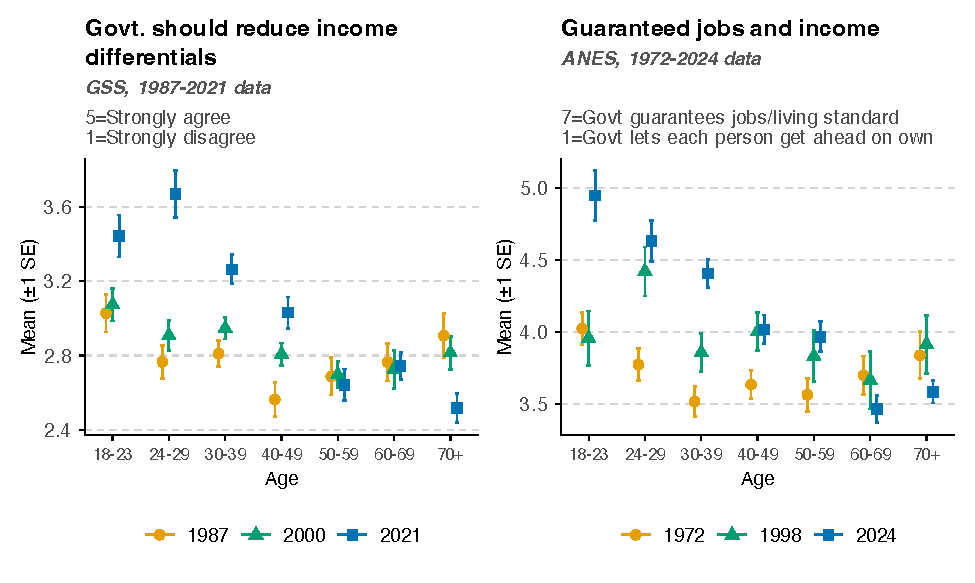
\includegraphics[width=0.88\linewidth]{figures/pair_headline_slide.pdf}
    \caption{\centering Age gradient in support for redistribution by survey year: GSS GOVEQINC (left) and ANES VCF0809 (right)}
\end{figure}

\end{frame}



\begin{frame}{Zero-sum and attribution beliefs over time}

\begin{figure}
    \centering
    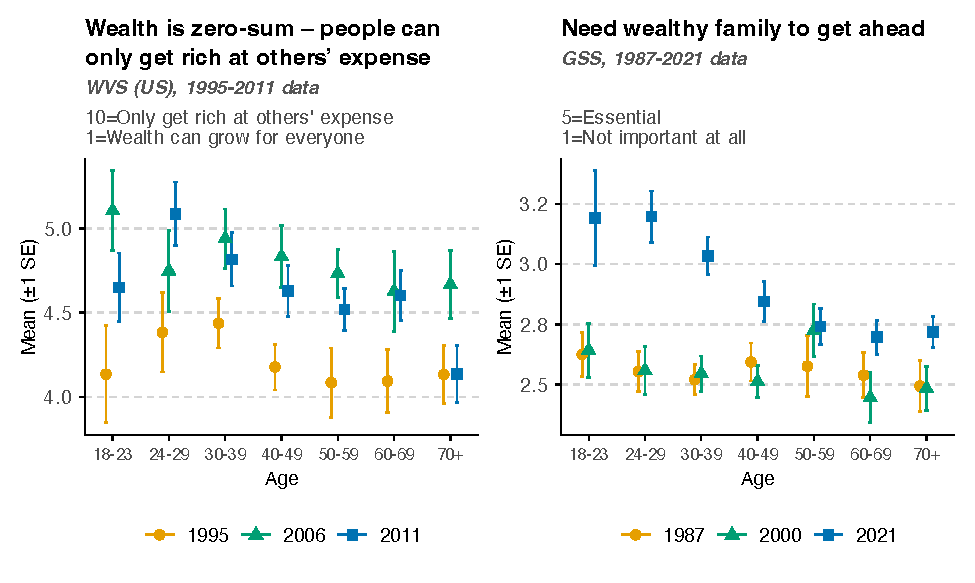
\includegraphics[width=0.88\linewidth]{figures/pair_zerosum_longrun_slide.pdf}
    \caption{\centering Age gradient in beliefs by survey year: WVS (US) E041 zero-sum wealth (left) and GSS OPWLTH need a wealthy family (right)}
\end{figure}

\end{frame}



\begin{frame}{Redistribution and belief gaps over time}

\begin{figure}
    \centering
    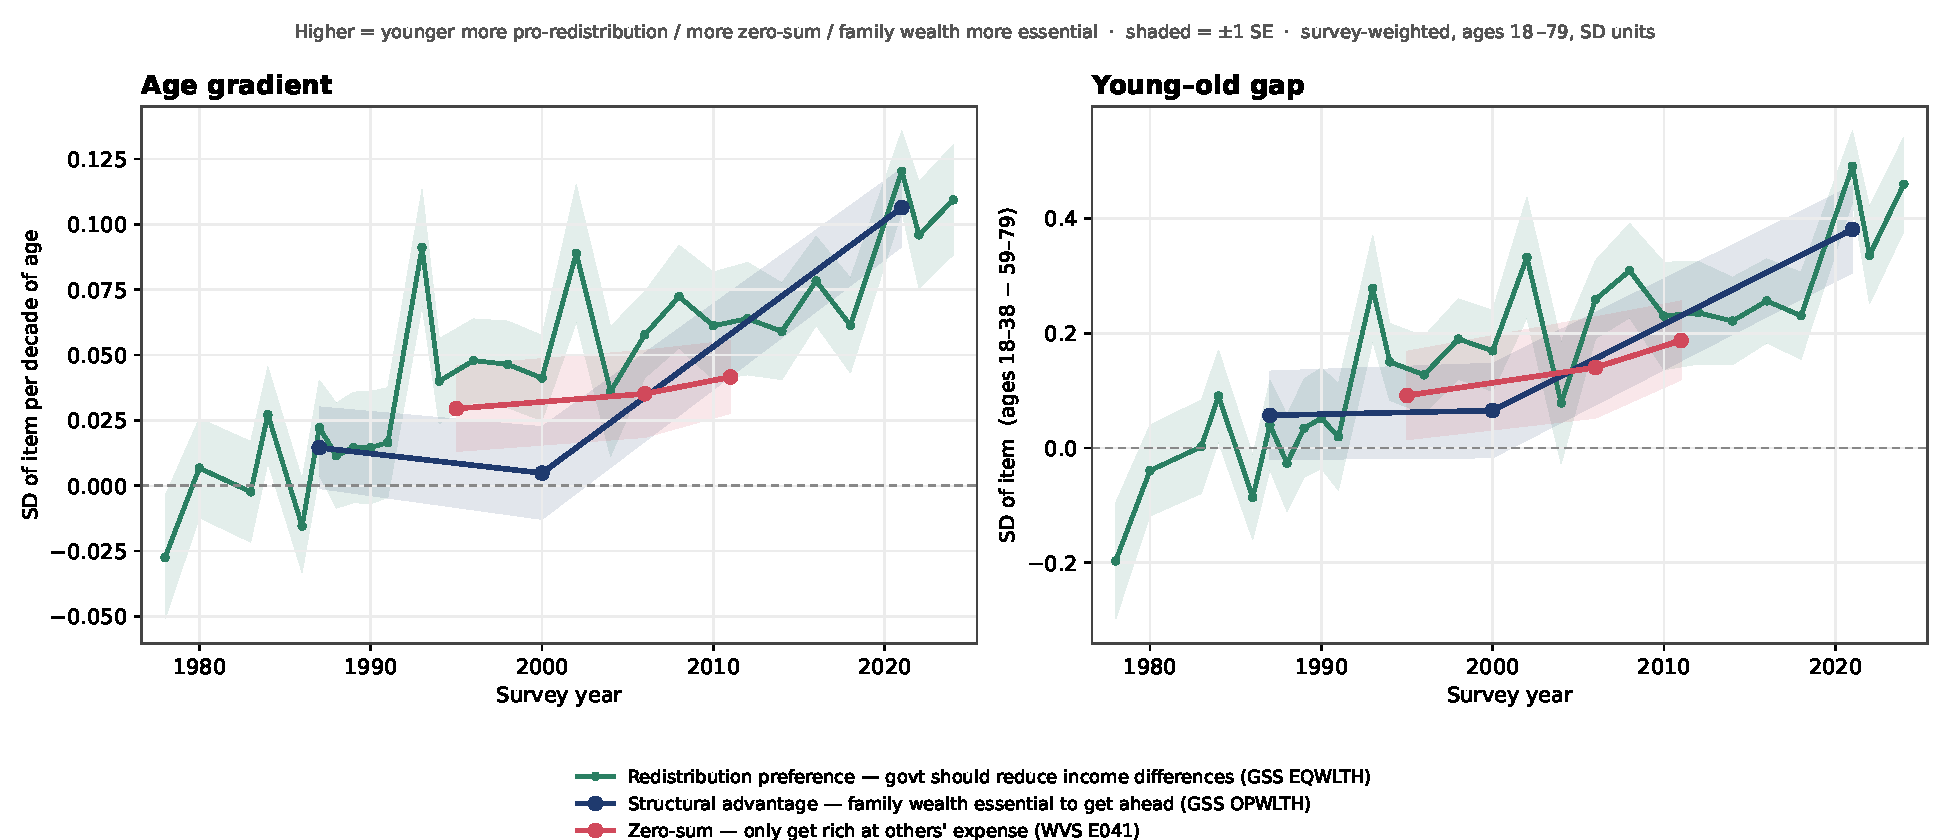
\includegraphics[width=\linewidth]{figures/fig_zerosum_vs_gap.pdf}
    \caption{\centering Young--old gap over time in redistribution preference (GSS EQWLTH) vs.\ zero-sum (WVS E041) and structural-advantage (GSS OPWLTH) beliefs, common SD units: age gradient (left) and 3-bin gap (right)}
\end{figure}

\end{frame}



\begin{frame}{Inequality, growth, housing and the age gradient}

\begin{figure}
    \centering
    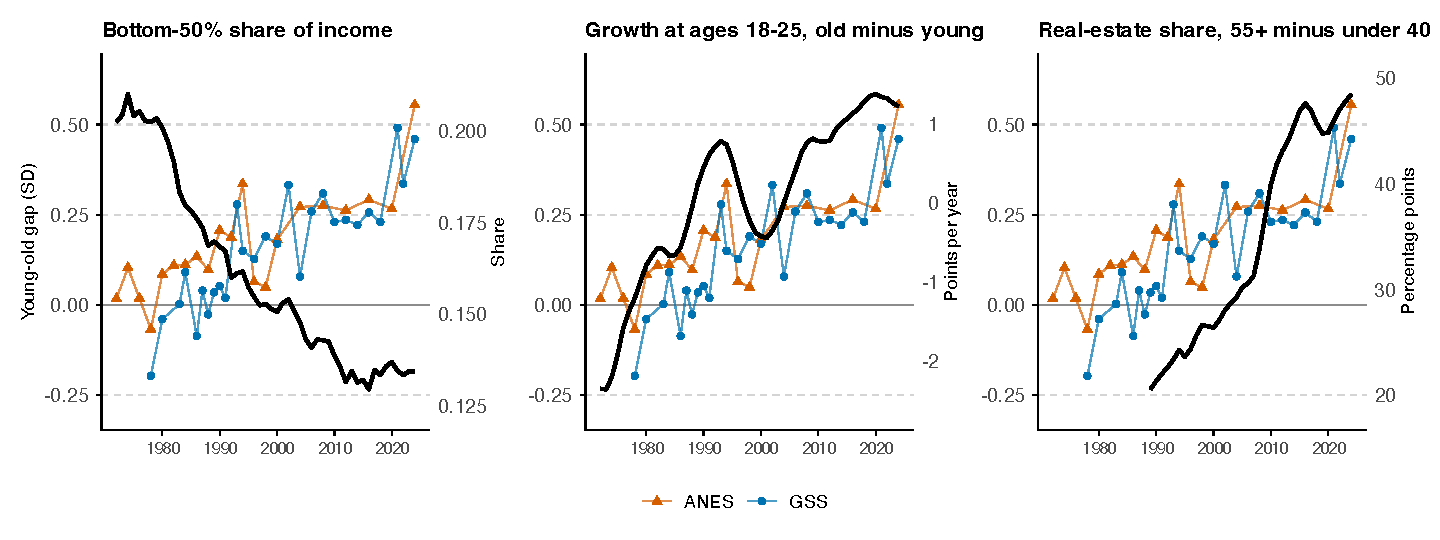
\includegraphics[width=\linewidth]{figures/fig_slide_ts_gradient_pair.pdf}
    \caption{\centering Age gradient in support for redistribution (GSS, ANES) vs.\ three US series, with correlations over survey years}
\end{figure}
\vspace{-0.6em}
{\tiny\centering Real estate: share of US household real estate held by households aged 55 and over minus the share held by those under 40, in percentage points (Federal Reserve Distributional Financial Accounts, quarterly from 1989). $r$ uses its annual mean.\par}

\end{frame}



\begin{frame}{The age gradient by race}

\begin{figure}
    \centering
    \begin{minipage}[c]{0.37\linewidth}\centering
        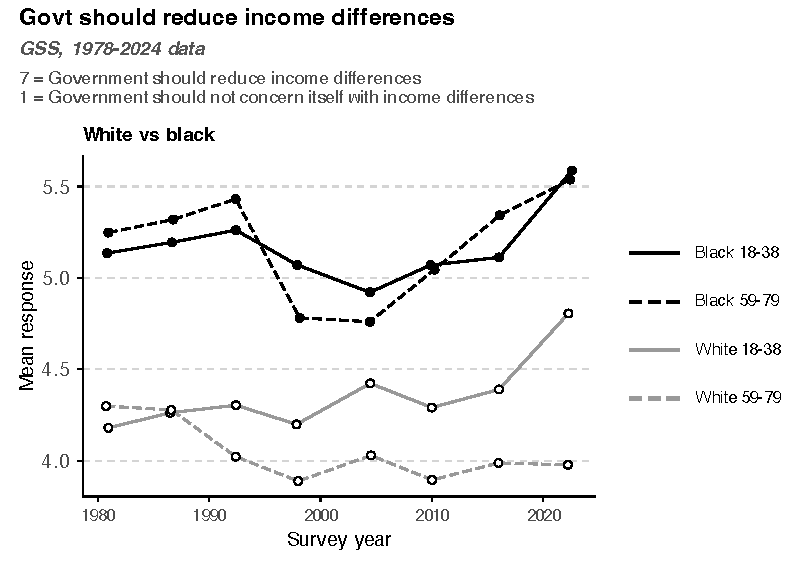
\includegraphics[width=\linewidth]{figures/fig_slide_race_EQWLTH.pdf}
    \end{minipage}\hfill
    \begin{minipage}[c]{0.61\linewidth}\centering
        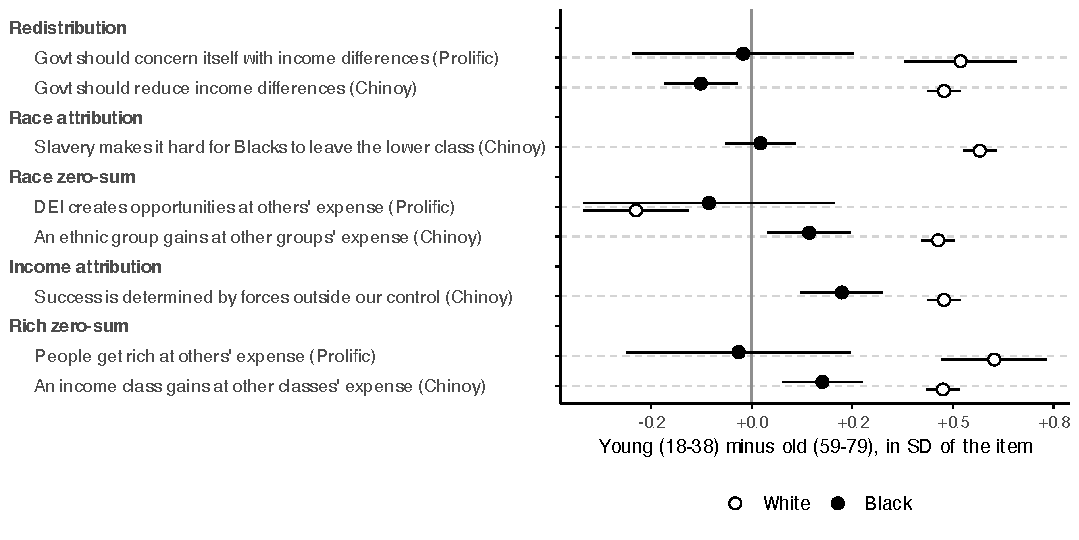
\includegraphics[width=\linewidth]{figures/xsec_gap_race.pdf}
    \end{minipage}
    \caption{\centering Left: GSS support for reducing income differences, white vs Black, ages 18--38 (solid) and 59--79 (dashed), six-year eras. Right: young--old gap (18--38 minus 59--79, SD) among white and Black respondents, Prolific and Chinoy items, 95\% intervals}
\end{figure}

\end{frame}



\begin{frame}{Formative growth and the gap across ANES states}

\begin{figure}
    \centering
    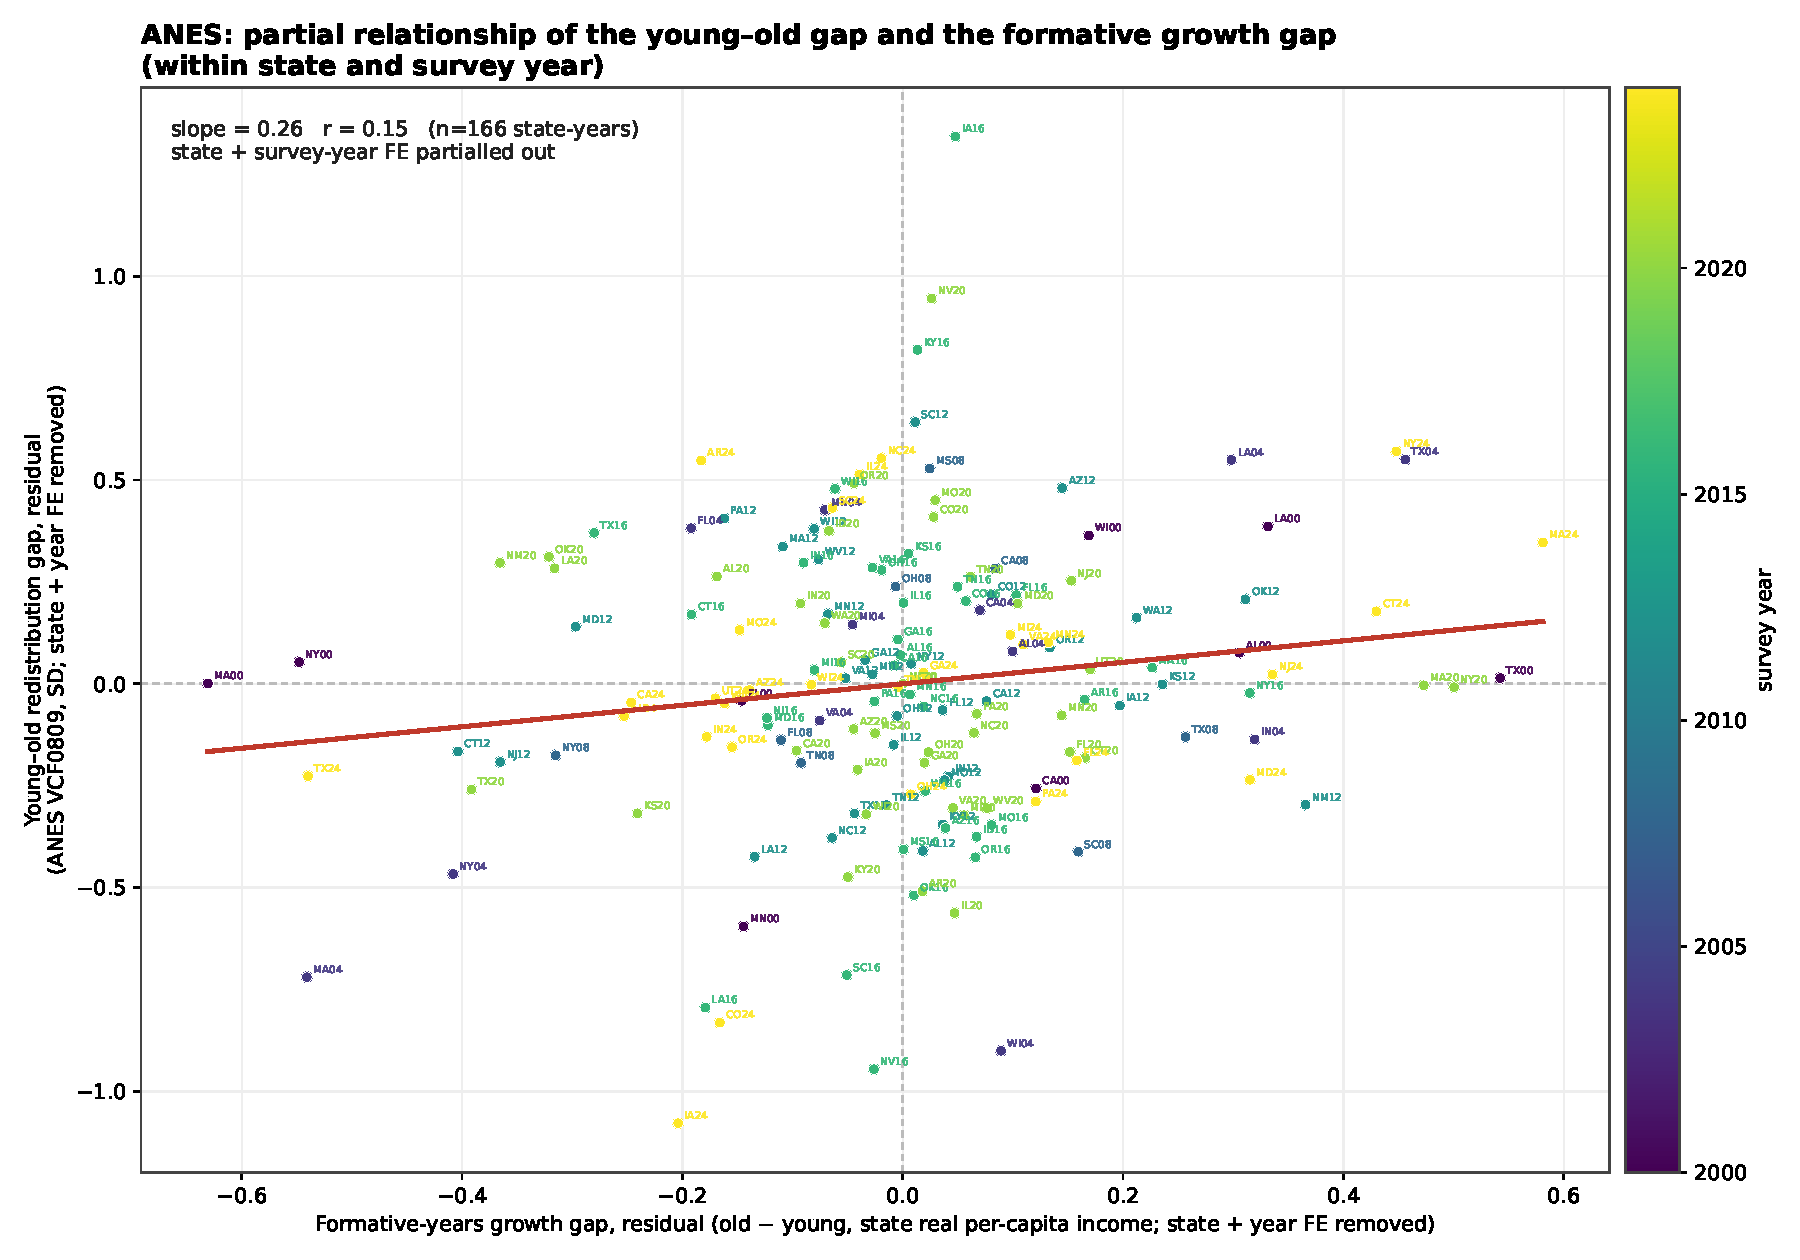
\includegraphics[width=0.7\linewidth]{figures/fig_anes_partial_corr.pdf}
    \caption{\centering ANES state $\times$ year: young--old redistribution gap vs.\ formative-years growth gap, net of state and year FE}
\end{figure}

\end{frame}



\begin{frame}{Formative-years growth and redistribution: ANES}

\begin{table}
    \centering
    \setbeamerfont{caption}{size=\footnotesize}
    \caption{ANES: support for redistribution on own-state formative-years growth}
    \vspace{-1.1em}
    {\tiny\setlength{\tabcolsep}{5pt}\renewcommand{\arraystretch}{0.82}
       \begin{tabular}{lcccc}
      \tabularnewline \midrule \midrule
      Dependent Variable: & \multicolumn{4}{c}{Support for redistribution (VCF0809)}\\
                                              & 0--20          & 18--25         & 0--20, $+$age          & 0--20, $+$cohort FE \\   
      Model:                                  & (1)            & (2)            & (3)                    & (4)\\  
      \midrule
      \emph{Variables}\\
      Own-state formative growth, ages 0--20  & -0.090$^{***}$ &                & 0.013                  & 0.016\\   
                                              & (0.012)        &                & (0.016)                & (0.021)\\   
      Own-state formative growth, ages 18--25 &                & -0.017$^{***}$ &                        &   \\   
                                              &                & (0.004)        &                        &   \\   
      Age                                     &                &                & -0.024$^{***}$         &   \\   
                                              &                &                & (0.003)                &   \\   
      Age$^2$                                 &                &                & 0.0002$^{***}$         &   \\   
                                              &                &                & ($3.4\times 10^{-5}$)  &   \\   
      \midrule
      \emph{Fixed-effects}\\
      State                                   & Yes            & Yes            & Yes                    & Yes\\  
      Survey year                             & Yes            & Yes            & Yes                    & Yes\\  
      Birth year (cohort)                     &                &                &                        & Yes\\  
      \midrule
      \emph{Fit statistics}\\
      Observations                            & 36,101         & 40,784         & 36,101                 & 36,101\\  
      R$^2$                                   & 0.02238        & 0.01688        & 0.03462                & 0.03816\\  
      Within R$^2$                            & 0.00473        & 0.00073        & 0.01719                & $3.44\times 10^{-5}$\\   
      \midrule \midrule
      \multicolumn{5}{l}{\emph{Clustered (State) standard-errors in parentheses}}\\
      \multicolumn{5}{l}{\emph{Signif. Codes: ***: 0.01, **: 0.05, *: 0.1}}\\
   \end{tabular}
\vspace{3pt}\par\centering{\setlength{\tabcolsep}{4pt}
\begin{tabular}{lcccc}
\multicolumn{1}{l}{\itshape Economic size (significant columns only):}
 & (1) & (2) & (3) & (4)\\
\midrule
Per $+1$\,SD of regressor ($\Delta$ outcome, SD) & $-0.081$ & $-0.028$ & -- & --\\
\quad as \% of the young--old gap & 33\% & 9\% & -- & --\\
\end{tabular}}
}
\end{table}

\end{frame}



\begin{frame}{Absolute mobility and redistribution: ANES}

\begin{table}
    \centering
    \setbeamerfont{caption}{size=\footnotesize}
    \caption{ANES: support for redistribution on own-state absolute mobility}
    \vspace{-1.1em}
    {\tiny\setlength{\tabcolsep}{5pt}\renewcommand{\arraystretch}{0.82}
       \begin{tabular}{lccc}
      \tabularnewline \midrule \midrule
      Dependent Variable: & \multicolumn{3}{c}{Support for redistribution (VCF0809)}\\
                                       & state$+$yr     & $+$age                  & $+$cohort FE \\   
      Model:                           & (1)            & (2)                     & (3)\\  
      \midrule
      \emph{Variables}\\
      Own-state absolute mobility (SD) & -0.095$^{***}$ & -0.003                  & -0.012\\   
                                       & (0.008)        & (0.016)                 & (0.063)\\   
      Age                              &                & -0.024$^{***}$          &   \\   
                                       &                & (0.004)                 &   \\   
      Age$^2$                          &                & 0.0002$^{***}$          &   \\   
                                       &                & ($4.11\times 10^{-5}$)  &   \\   
      \midrule
      \emph{Fixed-effects}\\
      State                            & Yes            & Yes                     & Yes\\  
      Survey year                      & Yes            & Yes                     & Yes\\  
      Birth year (cohort)              &                &                         & Yes\\  
      \midrule
      \emph{Fit statistics}\\
      Observations                     & 30,252         & 30,252                  & 30,252\\  
      R$^2$                            & 0.02219        & 0.02505                 & 0.02650\\  
      Within R$^2$                     & 0.00715        & 0.01006                 & $3.29\times 10^{-6}$\\   
      \midrule \midrule
      \multicolumn{4}{l}{\emph{Clustered (State) standard-errors in parentheses}}\\
      \multicolumn{4}{l}{\emph{Signif. Codes: ***: 0.01, **: 0.05, *: 0.1}}\\
   \end{tabular}
\vspace{3pt}\par\centering{\setlength{\tabcolsep}{4pt}
\begin{tabular}{lccc}
\multicolumn{1}{l}{\itshape Economic size (significant columns only):}
 & (1) & (2) & (3)\\
\midrule
Per $+1$\,SD of regressor ($\Delta$ outcome, SD) & $-0.095$ & -- & --\\
\quad as \% of the young--old gap & 45\% & -- & --\\
\end{tabular}}
}
\end{table}

\end{frame}



\begin{frame}{Formative-years growth relative to the nation: ANES}

\begin{table}
    \centering
    \setbeamerfont{caption}{size=\footnotesize}
    \caption{ANES: support for redistribution on state$-$national formative growth}
    \vspace{-1.1em}
    {\tiny\setlength{\tabcolsep}{5pt}\renewcommand{\arraystretch}{0.82}
       \begin{tabular}{lcccc}
      \tabularnewline \midrule \midrule
      Dependent Variable: & \multicolumn{4}{c}{Support for redistribution}\\
      Spec.:                               & 0--20   & 18--25  & 0--20, $+$age           & 0--20, $+$coh. \\   
      Model:                               & (1)     & (2)     & (3)                     & (4)\\  
      \midrule
      \emph{Variables}\\
      State$-$national growth, ages 0--20  & -0.011  &         & 0.019                   & 0.016\\   
                                           & (0.040) &         & (0.024)                 & (0.021)\\   
      State$-$national growth, ages 18--25 &         & 0.009   &                         &   \\   
                                           &         & (0.017) &                         &   \\   
      Age                                  &         &         & -0.023$^{***}$          &   \\   
                                           &         &         & (0.003)                 &   \\   
      Age$^2$                              &         &         & 0.0002$^{***}$          &   \\   
                                           &         &         & ($3.42\times 10^{-5}$)  &   \\   
      \midrule
      \emph{Fixed-effects}\\
      State                                & Yes     & Yes     & Yes                     & Yes\\  
      Survey year                          & Yes     & Yes     & Yes                     & Yes\\  
      Birth year (cohort)                  &         &         &                         & Yes\\  
      \midrule
      \emph{Fit statistics}\\
      Observations                         & 36,101  & 40,784  & 36,101                  & 36,101\\  
      R$^2$                                & 0.01775 & 0.01620 & 0.03461                 & 0.03816\\  
      \midrule \midrule
      \multicolumn{5}{l}{\emph{Clustered (State) standard-errors in parentheses}}\\
      \multicolumn{5}{l}{\emph{Signif. Codes: ***: 0.01, **: 0.05, *: 0.1}}\\
   \end{tabular}
\vspace{2pt}\par\centering{\itshape Economic size: no coefficient significant at 5\%.}
}
\end{table}

\end{frame}



\begin{frame}{Absolute mobility relative to the nation: ANES}

\begin{table}
    \centering
    \setbeamerfont{caption}{size=\footnotesize}
    \caption{ANES: support for redistribution on state$-$national absolute mobility}
    \vspace{-1.1em}
    {\tiny\setlength{\tabcolsep}{5pt}\renewcommand{\arraystretch}{0.82}
       \begin{tabular}{lccc}
      \tabularnewline \midrule \midrule
      Dependent Variable: & \multicolumn{3}{c}{Support for redistribution}\\
      Spec.:                              & state$+$yr     & $+$age                  & $+$coh. \\   
      Model:                              & (1)            & (2)                     & (3)\\  
      \midrule
      \emph{Variables}\\
      State$-$national abs. mobility (SD) & -0.060$^{***}$ & 0.010                   & -0.004\\   
                                          & (0.011)        & (0.013)                 & (0.019)\\   
      Age                                 &                & -0.024$^{***}$          &   \\   
                                          &                & (0.004)                 &   \\   
      Age$^2$                             &                & 0.0002$^{***}$          &   \\   
                                          &                & ($4.08\times 10^{-5}$)  &   \\   
      \midrule
      \emph{Fixed-effects}\\
      State                               & Yes            & Yes                     & Yes\\  
      Survey year                         & Yes            & Yes                     & Yes\\  
      Birth year (cohort)                 &                &                         & Yes\\  
      \midrule
      \emph{Fit statistics}\\
      Observations                        & 30,252         & 30,252                  & 30,252\\  
      R$^2$                               & 0.01746        & 0.02509                 & 0.02650\\  
      \midrule \midrule
      \multicolumn{4}{l}{\emph{Clustered (State) standard-errors in parentheses}}\\
      \multicolumn{4}{l}{\emph{Signif. Codes: ***: 0.01, **: 0.05, *: 0.1}}\\
   \end{tabular}
\vspace{3pt}\par\centering{\setlength{\tabcolsep}{4pt}
\begin{tabular}{lccc}
\multicolumn{1}{l}{\itshape Economic size (significant columns only):}
 & (1) & (2) & (3)\\
\midrule
Per $+1$\,SD of regressor ($\Delta$ outcome, SD) & $-0.061$ & -- & --\\
\quad as \% of the young--old gap & 18\% & -- & --\\
\end{tabular}}
}
\end{table}

\end{frame}



\begin{frame}{Inequality grown up with and redistribution: ANES}

\begin{table}
    \centering
    \setbeamerfont{caption}{size=\footnotesize}
    \caption{ANES: support for redistribution on the top-10\% income share grown up with}
    \vspace{-1.1em}
    {\tiny\setlength{\tabcolsep}{5pt}\renewcommand{\arraystretch}{0.82}
       \begin{tabular}{lcccc}
      \tabularnewline \midrule \midrule
      Dependent Variable: & \multicolumn{4}{c}{Y}\\
                                              & Top10 avg     & Top10 change  & avg $-$ nat & change $-$ nat \\   
      Model:                                  & (1)           & (2)           & (3)         & (4)\\  
      \midrule
      \emph{Variables}\\
      Top-10\% share, formative average (SD)  & 0.075$^{***}$ &               &             &   \\   
                                              & (0.011)       &               &             &   \\   
      Top-10\% share, formative change (SD)   &               & 0.079$^{***}$ &             &   \\   
                                              &               & (0.008)       &             &   \\   
      Formative average $-$ national (SD)     &               &               & 0.024       &   \\   
                                              &               &               & (0.023)     &   \\   
      Formative change $-$ national (SD)      &               &               &             & -0.012\\   
                                              &               &               &             & (0.010)\\   
      \midrule
      \emph{Fixed-effects}\\
      State                                   & Yes           & Yes           & Yes         & Yes\\  
      Survey year                             & Yes           & Yes           & Yes         & Yes\\  
      \midrule
      \emph{Fit statistics}\\
      Observations                            & 39,917        & 39,917        & 39,917      & 39,917\\  
      R$^2$                                   & 0.02235       & 0.02252       & 0.01783     & 0.01769\\  
      \midrule \midrule
      \multicolumn{5}{l}{\emph{Clustered (State) standard-errors in parentheses}}\\
      \multicolumn{5}{l}{\emph{Signif. Codes: ***: 0.01, **: 0.05, *: 0.1}}\\
   \end{tabular}
\vspace{3pt}\par\centering{\setlength{\tabcolsep}{4pt}
\begin{tabular}{lcccc}
\multicolumn{1}{l}{\itshape Economic size (significant columns only):}
 & (1) & (2) & (3) & (4)\\
\midrule
Per $+1$\,SD of regressor ($\Delta$ outcome, SD) & $+0.080$ & $+0.080$ & -- & --\\
\quad as \% of the young--old gap & 16\% & 35\% & -- & --\\
\end{tabular}}
}
\end{table}

\end{frame}



\begin{frame}{Perceived conflict between young and old}

\begin{figure}
    \centering
    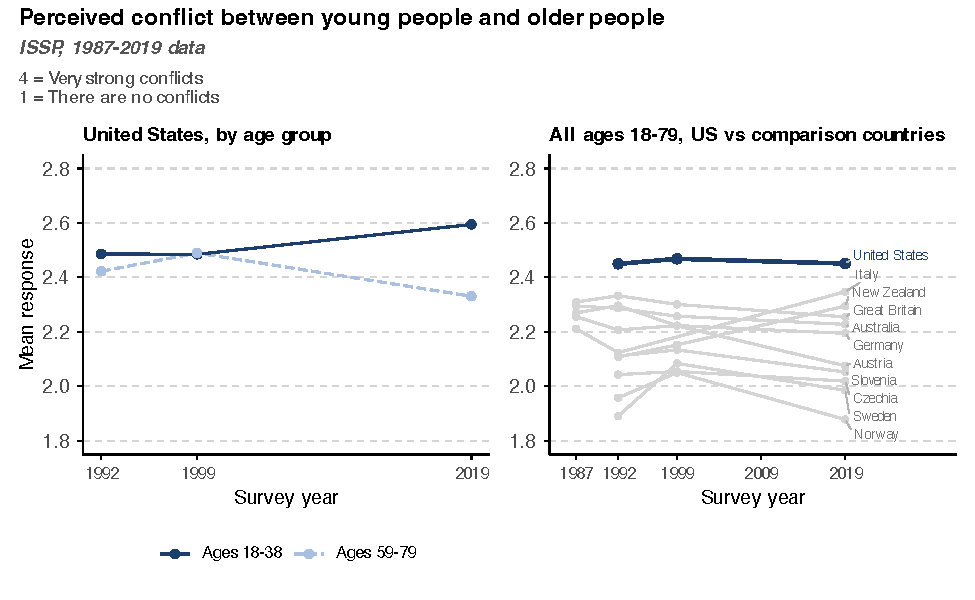
\includegraphics[width=0.78\linewidth]{figures/age_conflict.pdf}
    \caption{\centering Perceived conflict between young and older people (ISSP Social Inequality), mean on the 4-point scale (4 = very strong). Left: US, ages 18--38 and 59--79. Right: ages 18--79, US vs.\ rich democracies}
\end{figure}

\end{frame}



\begin{frame}{Social Security}

\begin{figure}
    \centering
    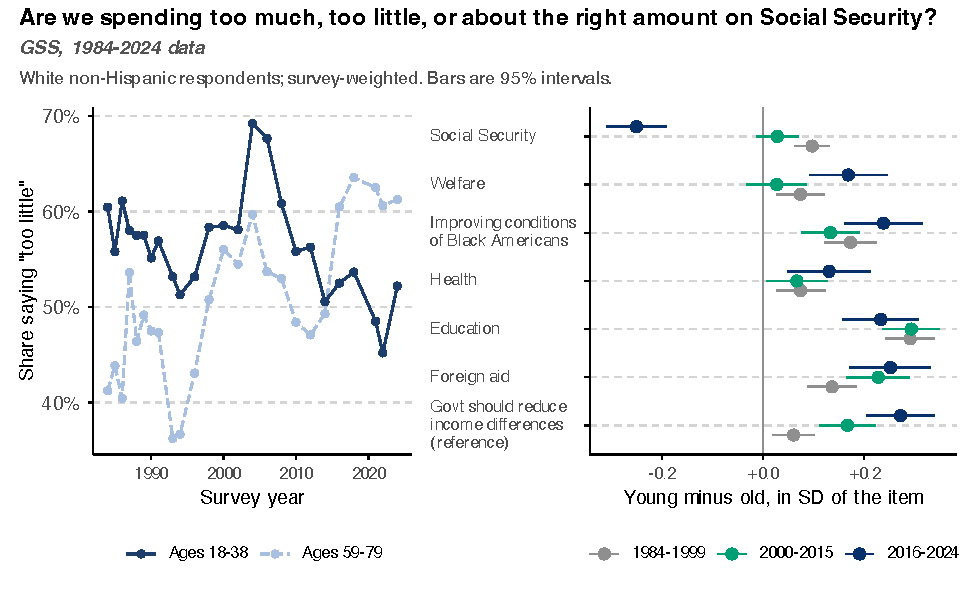
\includegraphics[width=0.72\linewidth]{figures/natsoc.pdf}
    \caption{\centering Left: share of white respondents saying Social Security spending is ``too little'', ages 18--38 and 59--79, by survey year. Right: young--old gap (SD) on each GSS spending item and the redistribution item, by era, 95\% intervals}
\end{figure}

\end{frame}


% \begin{frame}{Investigating drivers}

% Preliminary findings
% \begin{itemize}
%     \item Formative conditions alone do not explain it. Growth, inequality and mobility in a cohort's formative years predict at most 0.03 SD of a US gap of 0.3–0.7, and none of its rise. Chinoy's cross-country growth result does not replicate on our larger sample.
%     \item Institutional history does. On government responsibility, 11 of 28 advanced economies have a significant young-more-supportive gradient and 2 the reverse; in 33 countries with a socialist legacy it is 12 to 1 the other way. The US (−0.09) and UK (−0.12) are the steepest of 91.
% \end{itemize}

% \end{frame}



\begin{frame}{Investigating belief drivers}
% Investigating causality


Preliminary findings
\begin{itemize}
    \item Inequality, growth, and mobility alone do not explain any of the age gradient in cross-country analysis; the U.S. time series correlation is an outlier. 
    \item Trajectory of older Americans and non-formative-years placebo tests raise doubts about an imprinting story.
    \item Opposite age gradient on social security, emerging around 2020. 
    \item U.S. has highest perceived age conflict among rich democracies. Recently, the young perceive more conflict than the old.
    \item No age gap among Black Americans, only White/Hispanic.
    \item 3/4 of age gap survives within-party; not just higher polarization.
\end{itemize}
    
\end{frame}

\begin{frame}{Investigating belief drivers}

Why is the US unique? Possibilities:
\begin{itemize}
    \item Old-age benefits and the political power of the old
    \item Two-party bundling of cultural and economic positions (majoritarian vs. proportional system)
    \item Political entrepreneurs (Sanders, Trump)
    % Corbyn, Johnson. media narratives that place blame
    % Media segmentation: pre-2012 ANES access items show no differential gap; social-media batteries untested.
    % \item Social security and age representation in government
\end{itemize}
What explains sharp rise in gap post-2020?
\begin{itemize}
    \item Prominent billionaires reshaping society (Musk, Bezos)
    \item Racial justice salience (BLM movement)
    \item Affordability crisis (inflation, housing) and youth unemployment
    \item Government debt worries (social security more salient)
    \item Elderly presidential candidates in 2020 and 2024
\end{itemize}

\end{frame}

\begin{frame}{Investigating belief drivers}

Future analysis
\begin{itemize}
    \item Second survey wave
    \begin{itemize}
        \item A more comprehensive questionnaire pairing existing questions with govt. trust, religiosity, and race-related beliefs.
        \item In-depth measurement and differentiation of zero-sum/attribution beliefs. % which our current items partly confound
        \item An information provision or wording experiment generating exogenous belief variation.
    \end{itemize}
    \item Geographic and micro variation
    \begin{itemize}
        \item State and local-level age inequality measures: political representation (L2 voter files), policy tilt, real circumstances (housing, employment, etc.)
    \end{itemize}
    \item Text analysis
    \begin{itemize}
        \item Extracting zero-sum rich and zero-sum race narratives from Congressional speeches. Manifesto Project for cross-country.
    \end{itemize}
    % beliefs and preferences have moved a lot recently, so recent voter files (L2 and similar) and local exposure measures may give within-country variation.
\end{itemize}
    
\end{frame}

\end{document}

